\documentclass{../Common/Structure/doc_pdf}

\usepackage{pgffor}

\titleSubtitle{{\Huge\textit{Hypermedia project}}\\Prof. Franca Garzotto\\ \vspace{1cm}{\LARGE Design document}}{Version 1.0.0}
\pageHeader{Marco Travaglini, Francesco Zanoli, Francesco Di Febbo}

\begin{document}
\titleToc

\chapter{Abstract}
\thispagestyle{fancy}
The following document contains the IDM diagrams: C-IDM, L-IDM and P-IDM schemas of our website. We will also discuss about the scenario of a potential user and we show in the end a mockup explaining how the flow of the site works. We've used Balsamiq as prototyping tool for the interactive mockup and draw.io to built the IDM schemas. The wireframes inserted in this document will not contain the hyperlink of the interactive mockup. To completely use the potential of our mockup it is necessary to use the correspondent pdf.

\chapter{Graphical representation}
\thispagestyle{fancy}

{\centering 
C-IDM Schema
\vspace{1cm}
\begin{center}
	\includegraphics[width=\textwidth]{Clinic_C_IDM.jpg}
\end{center}}

\newpage

{\centering 
L-IDM Schema
\vspace{1cm}
\begin{center}
	\includegraphics[width=\textwidth]{Clinic_L_IDM.jpg}
\end{center}}

\newpage

{\centering 
P-IDM Schema
\vspace{1cm}
\begin{center}
	\includegraphics[width=\textwidth]{Clinic_P_IDM.jpg}
\end{center}}

%!!!!!!!!!! TODO controllare grammatica, scrivere scenario 3
\chapter{Scenarios}
\thispagestyle{fancy}
\section{Scenario 1}
Bob needs to do an electrocardiogram. Different friends suggested him to do it at Hospidif. Bob has never been to the clinic before and before take a decision he wants to get more information through the site www.hospidif.com.
From the homepage he clicks on the button Services. At this point he has to choose a specific area to filter all the available services.
He select then the cardiology area. Between the different he chooses the electrocardiogram  and accesses to the page with all the information concerning the service. Reading the description of the service he finds that there is just one location to access to this service. He clicks on the link "London Westminster". He reads all the information about the location and then he clicks on "How to reach the location". He finds out that the clinic is not too far away from his house. He decides to look for more information about the service so he goes back with the back button and returns to the service's page.
This time he clicks on the first doctor on the list. He opens then the doctor's description page. He reads all the informations about the medicine . He comes back again to the service's page and he repeats the passage for all the doctors. Bob is really interested in this service so he decides to arrange an appointment. To do so he clicks on the button area in the menu. He chooses the location of London Westminster by clicking on the button. he chooses again cardiology and he arrived on the area's detail page. At this point he can click on the Responsible Doctor, open the doctor's detail page and click on the button call.

\newpage

\section{Scenario 2}
Patrick used a few days ago the Hospidif's service. He is really satisfied about the treatment he received in the clinic and he decided to access to the site to read a few information about it. From the homepage he clicks on the button "Who we are". He reads all the information concerning the history of the clinic. He is also interested in witch new technology the clinic is studying at the moment so he clicks on the button "Project". finally he wants to see what is going on at the clinic  so he clicks on news in the menu. He finds a list of news concerning the clinic. He is really interested and he clicks on the first one to know more.

\newpage

\section{Scenario 3}

%!!!!!!!!!! TODO ricreare gli scenari
\chapter{Wireframes}
\thispagestyle{fancy}
\foreach\x in {1,5,6,7,29,41,75,76,119,120,148,158,117,184,186,189,198,200,204,207}{
	\begin{center}
		\includegraphics[page=\x, width=\textwidth]{../Mockup/Desktop/mockup2.pdf}
	\end{center}
	\vspace{0.7cm}
}

\appendix
\chapter{Appendix}
\section{Version History}
In the following are listed the differences between versions:
\begin{itemize}
	\item 1.0.0: first release
\end{itemize}
\end{document}
